\documentclass[a4paper, 10pt]{article}
\usepackage{graphicx} % Required for inserting images
\usepackage[utf8]{inputenc}
\usepackage[german]{babel}
\usepackage{geometry}
\usepackage{fancyhdr}
\usepackage{titlesec}
\usepackage{xcolor}
\usepackage{enumitem}
\usepackage{lipsum}
\usepackage{tcolorbox}
\usepackage{amsmath} % Für mathematische Formeln (optional)
\usepackage{xcolor}  % Für Farbdefinitionen
\usepackage{soul}    % Für Textmarkierung
\usepackage{verbatim}
\usepackage{listings}
%Seitenlayout
\geometry{top=2.5cm, left=2cm, right=2cm}

%Kopf- und Fußzeile
\pagestyle{fancy}
\fancyhf{}
\fancyhead[L]{\textbf{Compilerbau 2024/25}}
\fancyhead[R]{\textbf{Lena Thuy Trang Vo}}
\fancyfoot[C]{\thepage}

%Farben 
\definecolor{lightpastelblue}{rgb}{0.80, 0.92, 0.98}
\definecolor{darkpastelblue}{rgb}{0.60, 0.80, 0.90}

% Titel-Formatierung
\titleformat{\section}{\large\color{darkpastelblue}\bfseries}{}{0em}{}[\titlerule]
\titleformat{\subsection}{\color{darkpastelblue}\bfseries}{}{0em}{}

% Definition-Box
\newtcolorbox{definitionbox}{
  colback=lightpastelblue, % Hintergrundfarbe
  colframe=darkpastelblue, % Rahmenfarbe
  fonttitle=\bfseries,
  title=Definition,
  boxrule=0.8mm, % Dicke des Rahmens
  width=\textwidth, % Breite der Box
  before=\vspace{0.5cm}, % Abstand vor der Box
  after=\vspace{0.5cm}, % Abstand nach der Box
  sharp corners=south % Scharfe Ecken unten
}

\definecolor{lightblue}{rgb}{0.80, 0.92, 0.98}
% Befehl für das Hervorheben
\sethlcolor{lightblue} % Setze die Highlight-Farbe

\begin{document}

\begin{titlepage}
    \centering
    \vspace*{3cm}
    {\Huge \textbf{Einführung in den Compilerbau}}\\[1.5cm]
    {\large \textit{Lena Thuy Trang Vo}}\\[0.5cm]
    {\large \textit{Wintersemester 2024/25}}\\[2cm]

    \vfill
\end{titlepage}

\tableofcontents
\newpage

\section{Einführung}
Schnittstelle zwischen Programmiersprache und Maschine
\begin{itemize}
    \item \hl{Programmiersprache} ist gut für den Menschen handhabbar
    \begin{itemize}
        \item Smalltalk
        \item Java
        \item C++
    \end{itemize}

    \item \hl{Maschine} ist getrimmt auf
    \begin{itemize}
        \item Ausführungsgeschwindigkeit
        \item Preis/Chip-Fläche
        \item Energieverbrauch
        \item nur selten: leichte Programmierbarkeit 
    \end{itemize}
\end{itemize}

\subsection{Auswirkung von Compilern}
\begin{itemize}
    \item entscheidet über dem Benutzer \hl{zugängliche} Rechenleistung
    \item Compiler entscheiden maßgeblich über die \textbf{Effizienz und Leistung} eines Programms auf der Zielhardware
    \item beeinflussen nicht nur die \textbf{Geschwindigkeit der Programmausführung}, sondern auch den \textbf{Speicherbedarf} und die \textbf{Energieeffizienz}
\end{itemize}
\subsection{Programmiersprachen}
\textbf{hohe Ebene: Smalltalk, Java, C++}
\begin{lstlisting}[language=Java]
    let
        var i : Integer;
    in
        i := i + 1;
\end{lstlisting}

\noindent\textbf{mittlere Ebene: Assembler}
\begin{lstlisting}
    LOAD    R1; (i)
    LOADI   R2, 1
    ADD     R1 R1, R2
    STORE   R1, (i)
\end{lstlisting}
\textbf{niedrige Ebene: Maschinensprache}
\begin{lstlisting}
    0110000100000110
    0111001001000001 
    1011000100010010 
    1001000100000110
\end{lstlisting}

\subsection{Unterschiedliche Abstraktionsebenen}
\begin{itemize}
    \item auf unteren Ebenen immer \textbf{feinere Beschreibung}
    \item immer näher an Zielmaschine (Hardware)
    \item Details werden von Compiler hinzugefügt
    \begin{itemize}
        \item durch verschiedenste Algorithmen
        \begin{itemize}
            \item \hl{Analyse von Programmeigenschaften}
            \item \hl{Verfeinerung der Beschreibung durch Synthese}
        \end{itemize}
    \end{itemize}
    \item Höhere Ebenen \textbf{erleichtern die Entwicklung komplexer Logik}, während niedrigere Ebenen \textbf{maximale Kontrolle} über die Hardware bieten
\end{itemize}
\section{Auswirkungen der Zielmaschine}

\subsection{Einfach: Henessy \& Patterson DLX}
\begin{figure}[h]
    \centering
    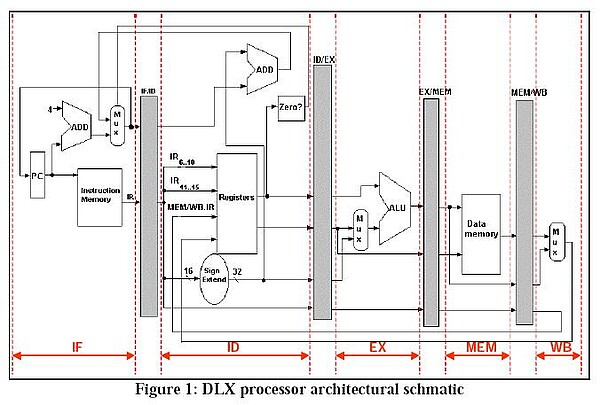
\includegraphics[width=0.5\linewidth]{/Users/lenavo/Desktop/3.Semester/Compilerbau/img/comp1.jpg}
    \caption{DLX-Prozessor}
    \label{fig:enter-label}
\end{figure}
\begin{itemize}
    \item ist eine \textbf{Reduced Instruction Set Computer} (RISC) Architektur, die auf \hl{Einfachheit} und \hl{Effizienz} ausgelegt ist
    \item basiert auf einem \textbf{Load/Store-Design}, bei dem \hl{alle Operationen auf Register beschränkt} sind mit Ausnahme von Lade- und Speicheroperationen
    \item die DLX-Architektur verwerndet eine \textbf{32-Bit-Datenbreite} und bietet 32 allgemeine Register, die jeweils 32 Bit breit sind
    \item implementiert eine \textbf{fünfstufige Instruktionspipeline}, die aus den Phasen \hl{Instruction Fetch} (IF), \hl{Instruction Decode} (ID), \hl{Execution} (EX), \hl{Memory Access} (MEM) und \hl{Write Back} (WB) besteht
\end{itemize}
\subsection{Komplizierter: Analog Devices TigerSHARC}

\begin{figure}[h]
    \centering
    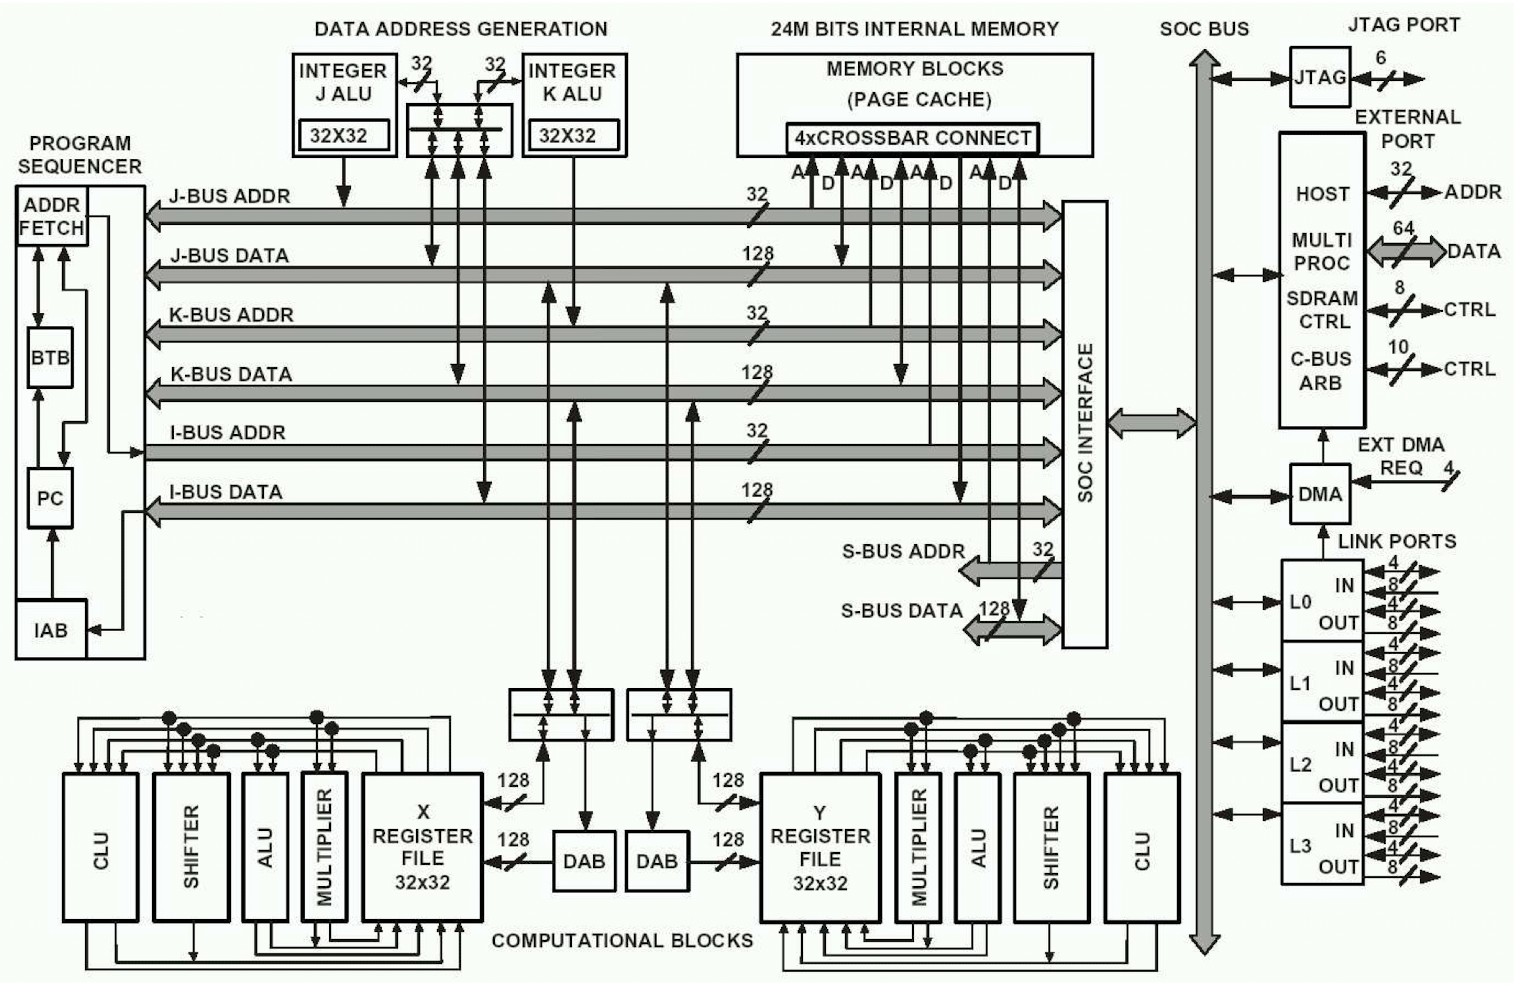
\includegraphics[width=0.5\linewidth]{/Users/lenavo/Desktop/3.Semester/Compilerbau/img/comp2.png}
    \caption{Analog Devices TigerSHARC}
    \label{fig:enter-label}
\end{figure}
\begin{itemize}
    \item ist ein leistungsstarker \textbf{digitaler Signalprozessor} (DSP), der für anspruchsvolle Anwendungen entwickelt wurde
    \item kann bis zu \hl{vier Instruktionen} pro Taktzyklus ausführenm was eine \hl{hohe Parallelität bei der Verarbeitung} ermöglicht
    \item  ist für \hl{Hochleistungs-Multiprocessing-Anwendungen} ausgelegt, wie z.B. Motorsteuerung, Energiemanagement, Prozesssteuerung und Sicherheitssysteme
    \item Kombination aus \textbf{hoher Ausführungsgeschwindigkeit}, \textbf{flexibler Datenverarbeitung} und \textbf{robuster Speicherverwaltung}
\end{itemize}
\subsection{Problematisch: IBM/Sony Cell Processor}
\begin{figure}[h]
    \centering
    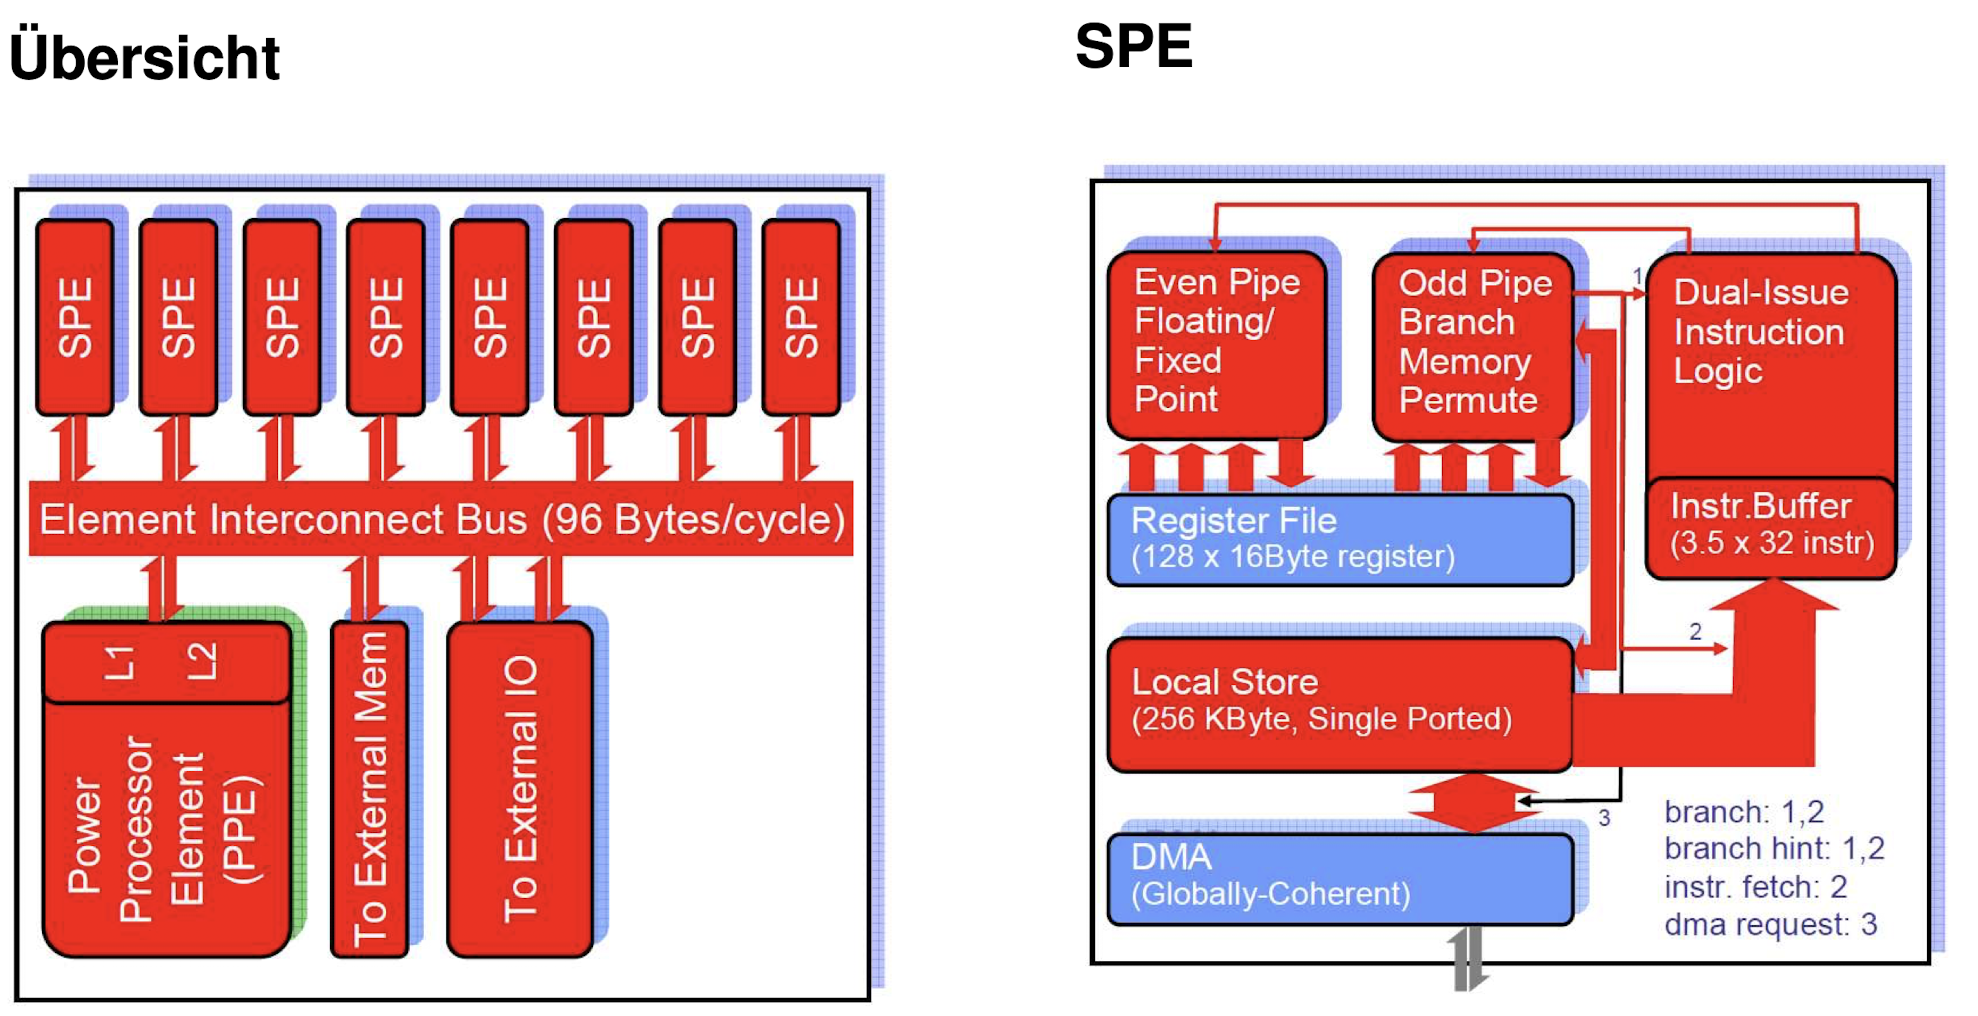
\includegraphics[width=0.6\linewidth]{/Users/lenavo/Desktop/3.Semester/Compilerbau/img/comp3.png}
    \caption{IBM/Sony Cell Processor}
    \label{fig:enter-label}
\end{figure}

\begin{itemize}
    \item ist eine innovative Prozessorarchitektur, die von \textbf{IBM}, \textbf{Sony} und \textbf{Toshiba} entwickelt wurde
    \item der zentrale Steuerprozessor basiert auf der \hl{64-Bit-PowerPC-Architektur} und kann \hl{zwei Threads gleichzeitig} verarbeiten
    \item parallele Verarbeitung
    \item in Ps3
\end{itemize}

\subsection{Spezialisierte Anforderungen an CPUs}
Je nach Anwendungsgebiet mehr oder weniger wichtig...
\begin{itemize}
    \item \hl{Rechenleistung} (hoch/niedrig):
    \begin{itemize}
        \item Anwendungen wie KI, Gaming oder CAD erfordern hohe Rechenleistung, während einfache Büroanwendungen weniger anspruchsvoll sind
    \end{itemize}

    \item \hl{Datentypen} (Gleitkomma, ganzzahlig, Vektoren):
    \begin{itemize}
        \item wissenschaftliche Berechnungne benötigen oft Gleitkommaoperationen, während Grafikverarbeitung von Vektorenoperationen profitiert
    \end{itemize}

    \item \hl{Operationen} (Multiplikationen, MACs):
    \begin{itemize}
        \item DSPs und Grafikprozessoren nutzen häufig MACs für schnelle Berechnungen in Signalverarbeitung und Rendering
    \end{itemize}

    \item \hl{Speicherbandbreite} (parallele Speicherzugriffe):
    \begin{itemize}
        \item hohe Speicherbandbreite ist entscheidend für Anwendungenm die große Datenmengen verarbeitenm wie Videobearbeitung oder Simulationen
    \end{itemize}

    \item \hl{Energieeffizienz}:
    \begin{itemize}
        \item in mobilen Geräten entscheident, um die Akkulaufzeit zu maximieren
    \end{itemize}

    \item \hl{Platzbedarf} (für den Prozessorchip):
    \begin{itemize}
        \item in eingebetteten Systemen und mobilen Geräten ist der Platzbedarf des Prozessors ein wichtiger Faktor
    \end{itemize}
\end{itemize}
... können häufig nur durch spezialisierte Prozessoren erfüllt werden\\[3mm]
$\longrightarrow$ \textbf{benötigen passende Compiler}

\subsection{Technologie}
\begin{itemize}
    \item Taktfrequenz von Prozessoren nur \textbf{mit Mühe steigerbar} 
    \item Trend geht weg von \textbf{hochgetakten Einzelprozessoren} hin zu vielen, aber langsameren Prozessoren
    \item um die Vorteile von Mehrkern-CPUs und GPUs zu nutzen, wurden verschiedene \hl{parallele Programmiermodelle} entwickelt:
    \begin{itemize}
        \item \textbf{OpenMP:} Mehr-Kern-CPUs
        \item \textbf{NVidia CUDA:} GPUs
        \item \textbf{OpenCL:} Heterogene Systeme (GPUs + CPUs, experimentell auch schon FPGAs)
    \end{itemize}
    \item aber noch wenig abstrakt
    \begin{itemize}
        \item Entwickler müssen \textbf{explizit angeben}, wie Aufgaben parallelisiert werden sollen, was \hl{komplex} und \hl{fehleranfällig} sein kann

    \end{itemize}
    \item keine automatische Parallelisierung!
\end{itemize}
\textbf{Anwendungsgebiet: Machine Learning}
\begin{itemize}
    \item Parallelisierung ist besonders wichtig im Bereich des maschinellen Lernens
    \item Frameworks wie TensorFlow XLA und Glow nutzen parallele Berechnungen, um komplexe Modelle effizienter zu trainieren und auszuführen
\end{itemize}

\section{Aufbau von Compilern}
\begin{itemize}
    \item Vorgehen: Bearbeitung in \textbf{mehreren Phasen}
    \item \hl{Zwischendarstellungen} werden verwendet, um Informationen zwischen diesen Phasen auzutauschen
\end{itemize}
\begin{figure}[h]
    \centering
    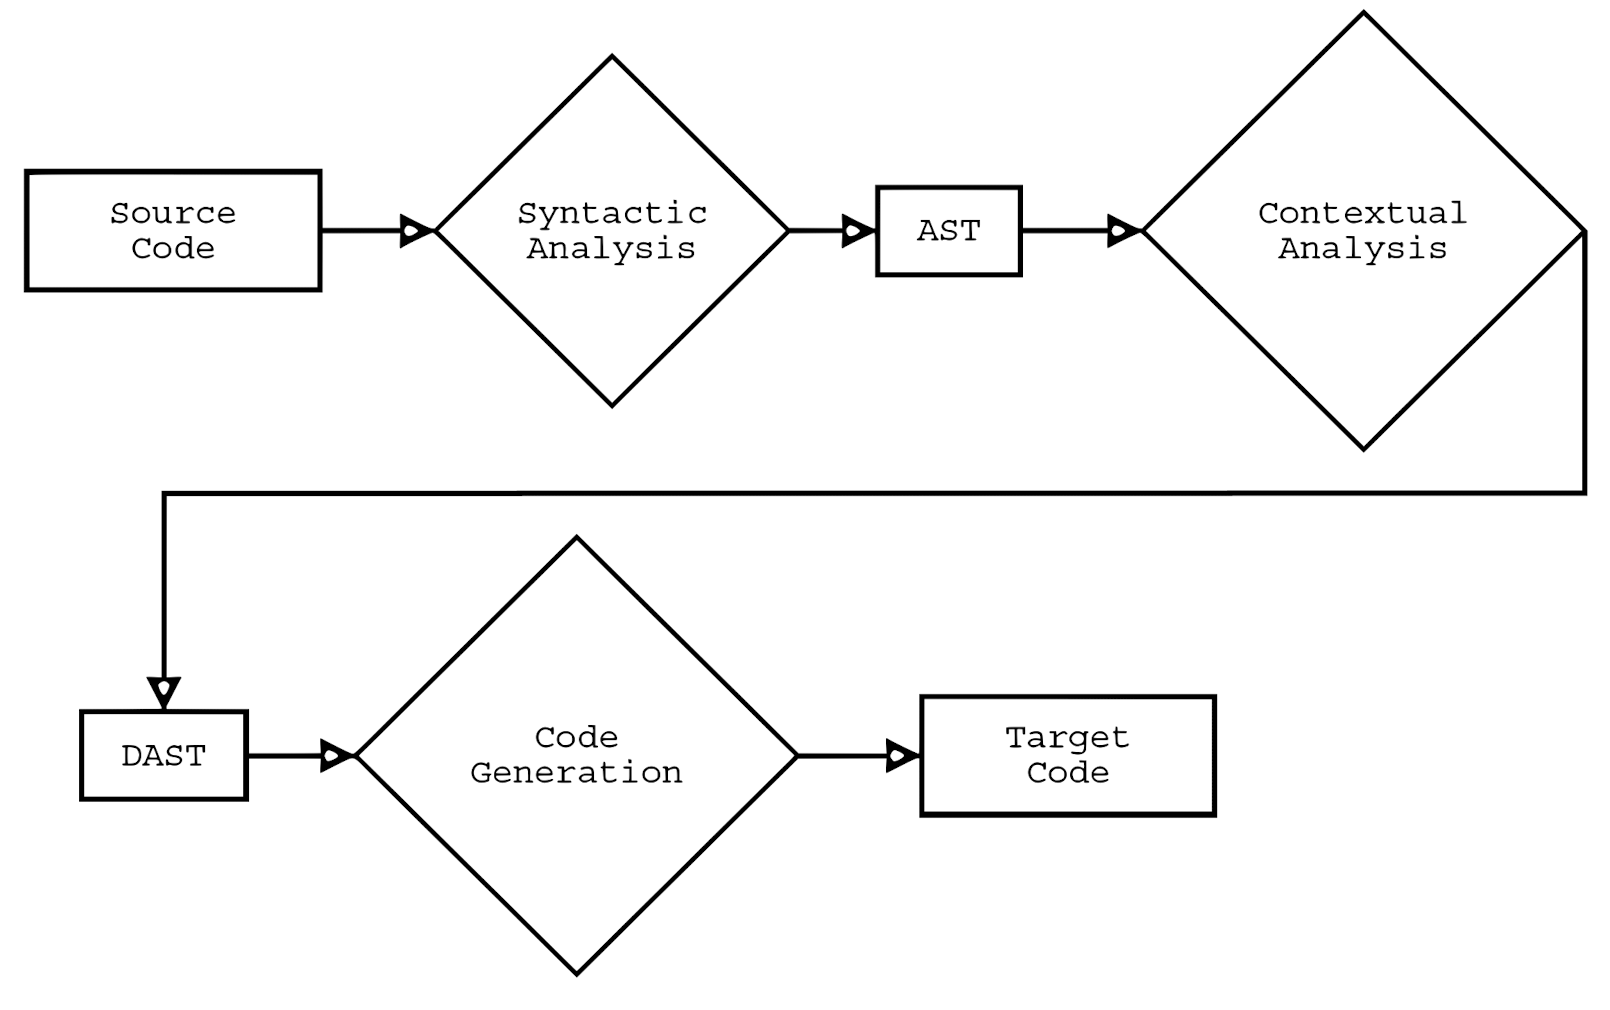
\includegraphics[width=0.4\linewidth]{/Users/lenavo/Desktop/3.Semester/Compilerbau/img/comp4.png}
    \caption{Vorgehen}
    \label{fig:enter-label}
\end{figure}
\subsection{Syntaxanalyse}
\begin{itemize}
    \item folgt auf die lexikalische Analyse und \textbf{überprüft}, ob der \textbf{Quellcode den Syntaxregeln} der jeweiligen Programmiersprache entspricht
    \item stellt sicher, dass der Quellcode grammatikalisch korrekt ist
    \item wenn der Code den Regeln entspricht, wird ein \hl{Syntaxbaum} erstellt
    \begin{itemize}
        \item dieser Baum repräsentiert die \hl{hierarchische Struktur} des Codes und dient als Grundlage für die nachfolgenden Phasen wie die s\hl{emantische Analyse} und \hl{Optimierung}
        \item Baum dient als \textbf{Zwischendarstellung für den Informationsaustausch} zwischen den verschiedenen Phasen des Compilers.
    \end{itemize}
\end{itemize}
\begin{figure}[h]
    \centering
    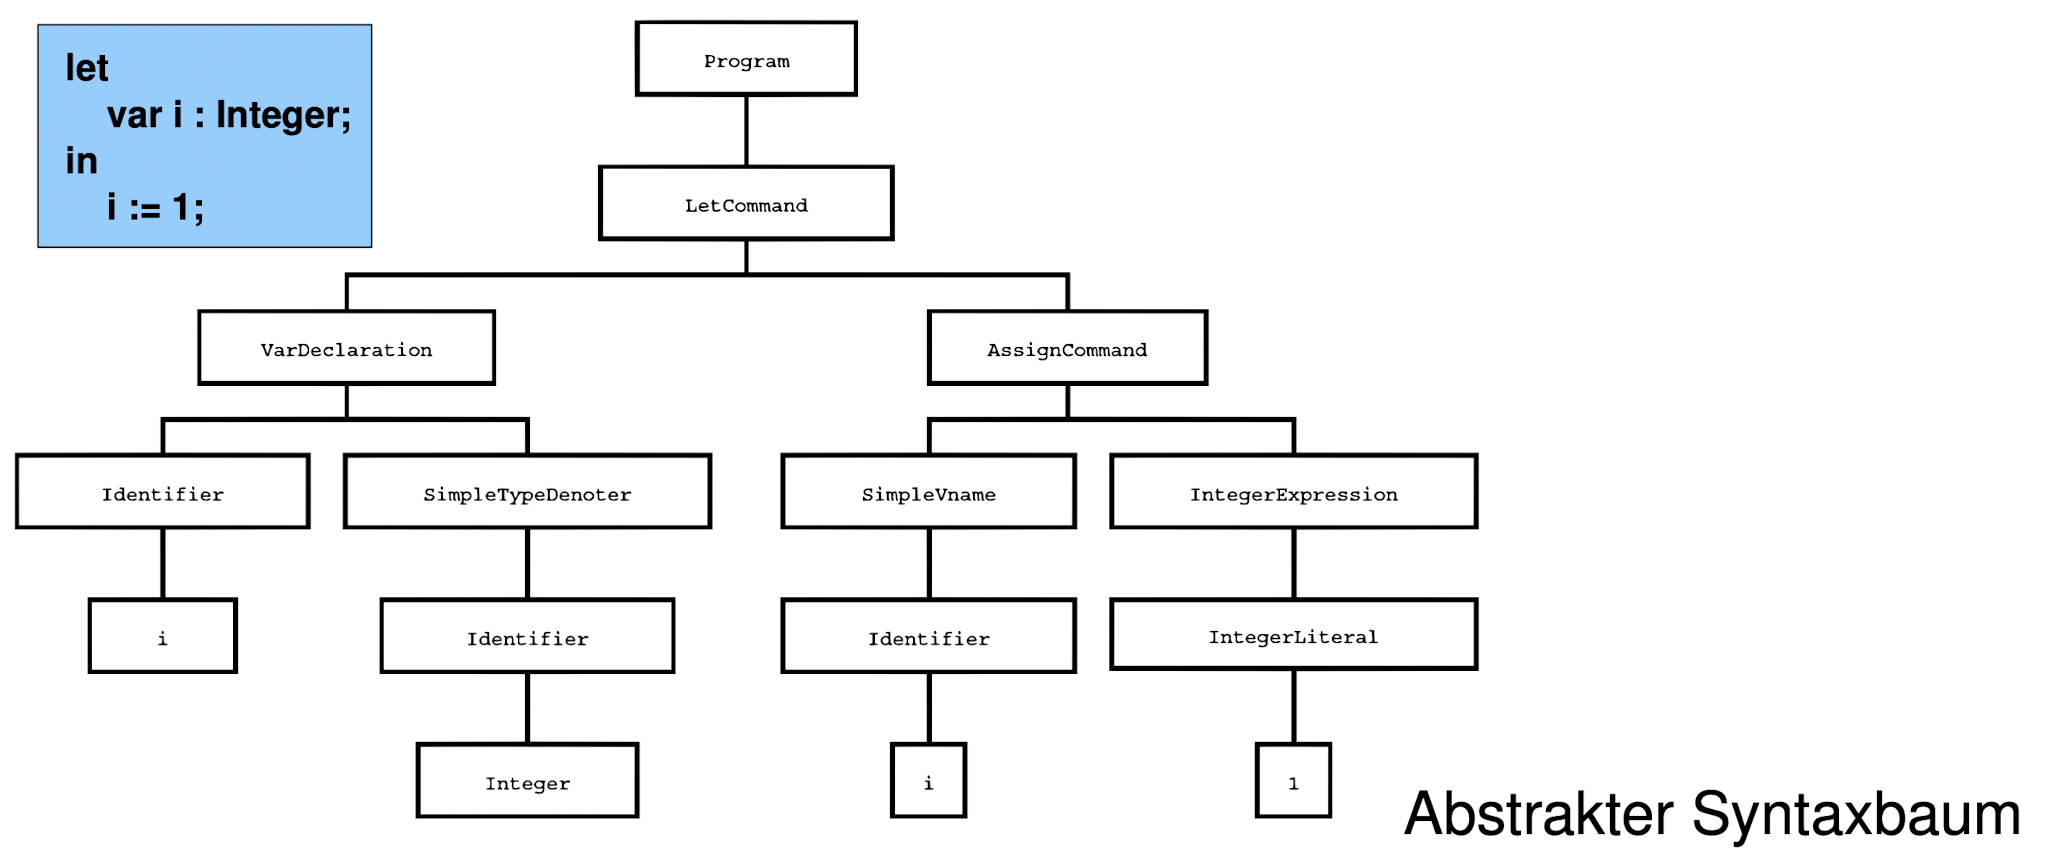
\includegraphics[width=0.7\linewidth]{/Users/lenavo/Desktop/3.Semester/Compilerbau/img/comp5.png}
    \caption{Syntaxbaum}
    \label{fig:enter-label}
\end{figure}

\subsection{Kontextanalyse}
\begin{itemize}
    \item auch als \textbf{semantische Analyse} bekannt
    \item überprüft, ob alle verwendeten Variablen \hl{korrekt deklariert} wurden
    \item stellt sicher, dass jede Variable vor ihrer Verwendung definiert ist und dass \textbf{keine Mehrfachdeklarationen} im selben Gültigkeitsbereich vorhanden sind
    \item bestimmt die \hl{Datentypen aller Ausdrücke} im Programm.
    \begin{itemize}
        \item \hl{Überprüfung von Typkompatibilität} bei Operationen und Zuweisungen, um sicherzustellen, dass beispielsweise keine Ganzzahlen mit Zeichenketten addiert werden
    \end{itemize}
\end{itemize}
\begin{figure}[h]
    \centering
    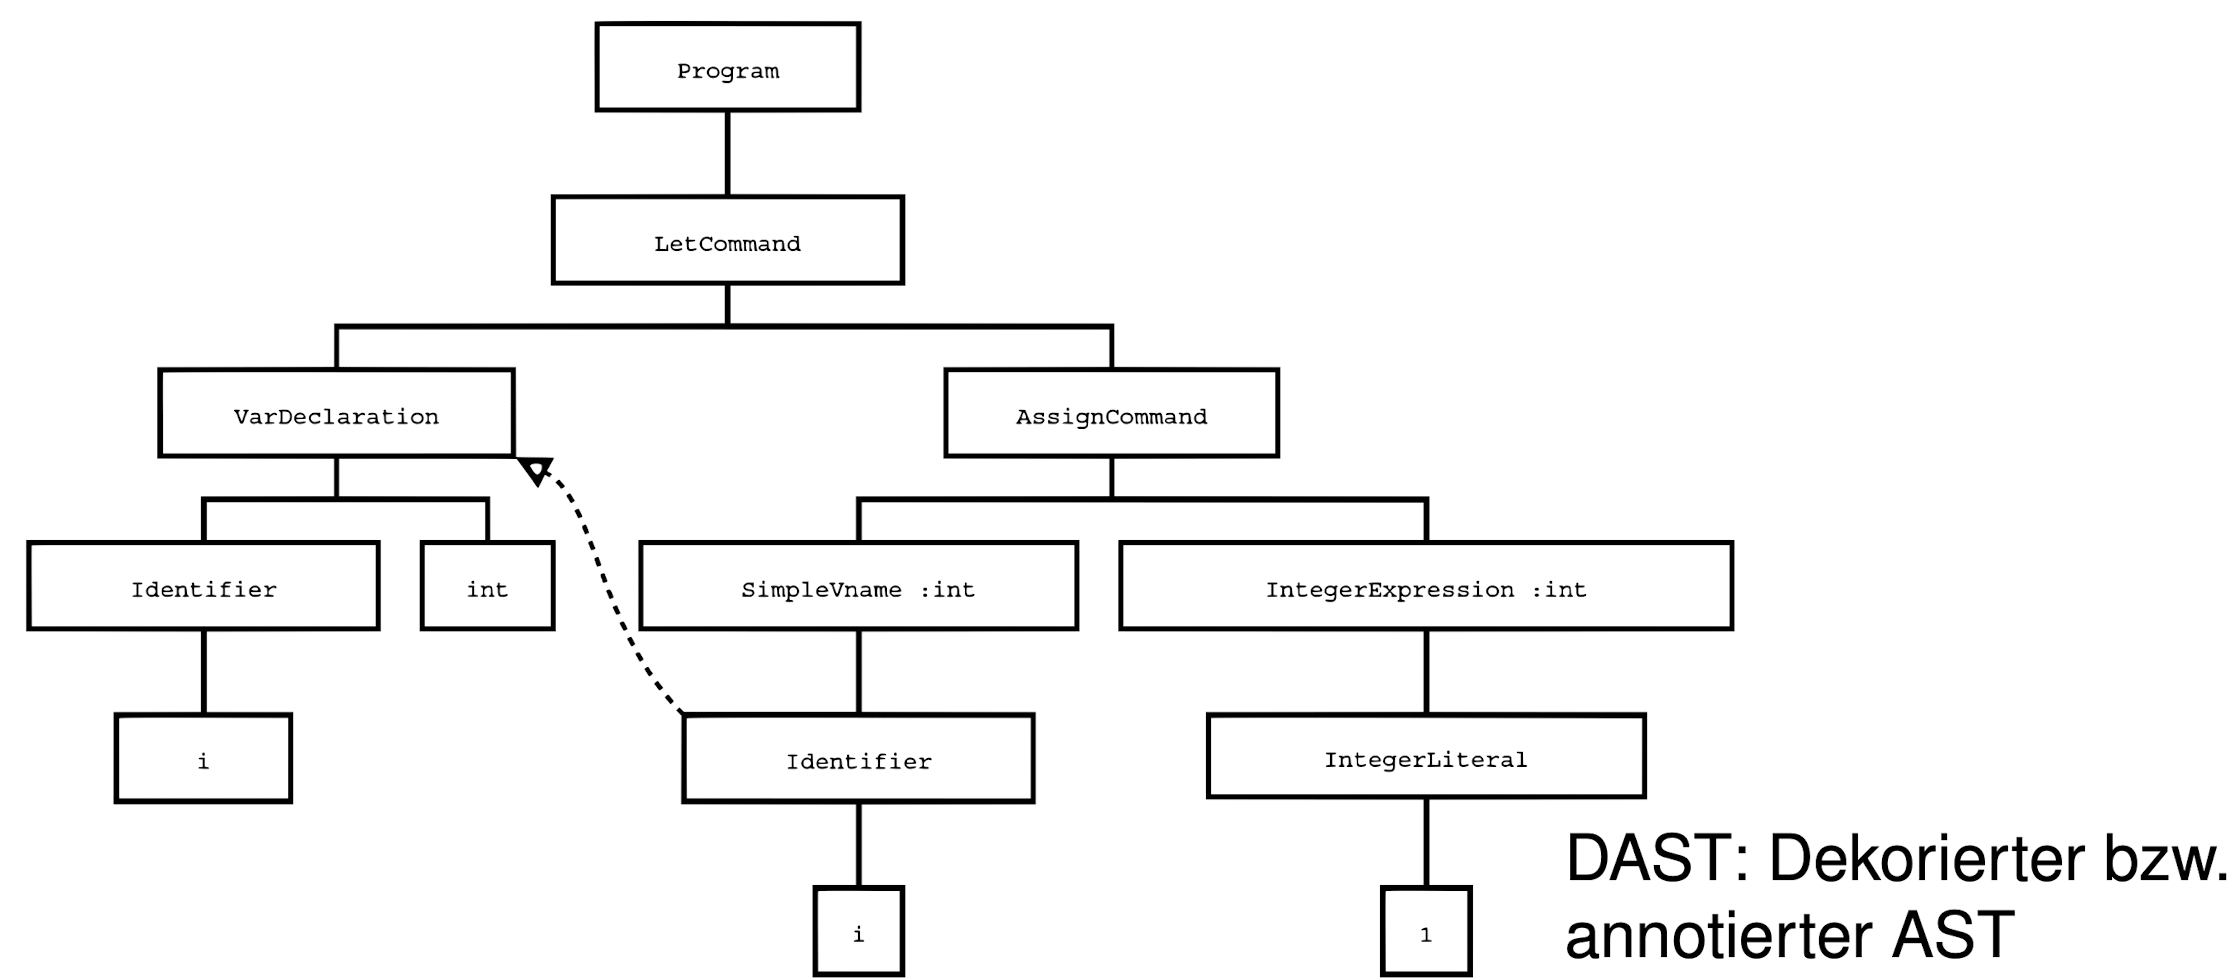
\includegraphics[width=0.6\linewidth]{/Users/lenavo/Desktop/3.Semester/Compilerbau/img/comp6.png}
    \caption{DAST}
    \label{fig:enter-label}
\end{figure}

\subsection{Code-Erzeugung}
\begin{itemize}
    \item Programm ist \hl{syntaktisch} und \hl{kontextuell} korrekt
    \item Übersetzung in Zielsprache
    \begin{itemize}
        \item Maschinensprache
        \item Assembler
        \item C
        \item andere Hochsprache
    \end{itemize}
    \item Zuweisung von \textbf{DAST-Teilen zu Instruktionen}
    \item Handhabung von Variablen
    \begin{enumerate}
        \item \hl{Deklaration:} Reserviere Speicherplatz für eine Variable
        \item \hl{Verwendung:} Referenziere immer den zugeordneten Speicherplatz
    \end{enumerate}
\end{itemize}
\begin{figure}[h]
    \centering
    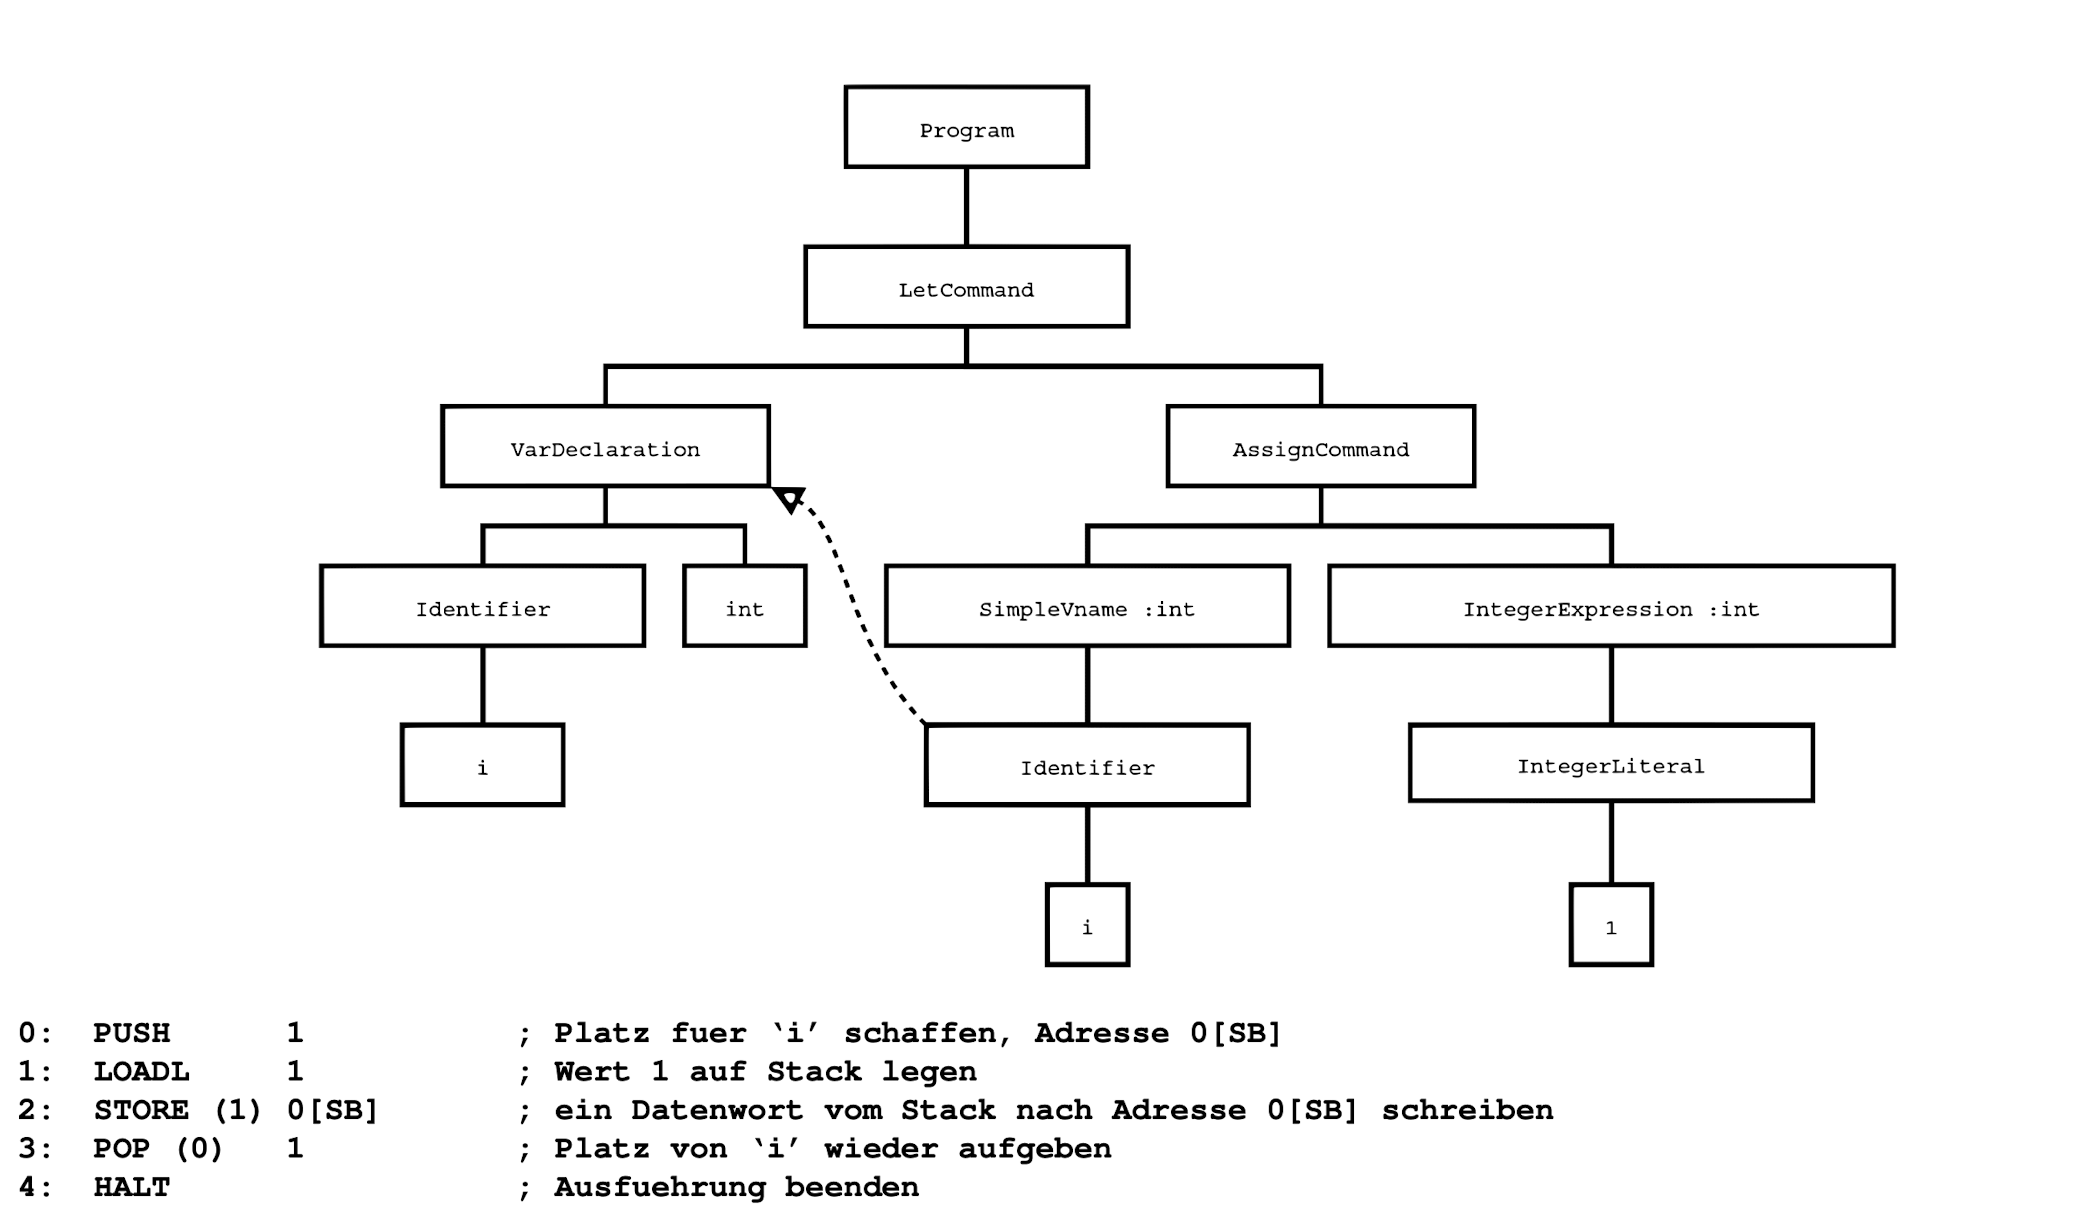
\includegraphics[width=0.8\linewidth]{/Users/lenavo/Desktop/3.Semester/Compilerbau/img/comp7.png}
    \caption{Code-Erzeugung}
    \label{fig:enter-label}
\end{figure}
\section{Optimierung}
\subsection{Optimierender Compiler}
\begin{figure}[h]
    \centering
    
\includegraphics[width=0.7\linewidth]{/Users/lenavo/Desktop/3.Semester/Compilerbau/img/comp8.png}
    \label{fig:enter-label}
\end{figure}
\begin{itemize}
    \item \hl{Front-End:} Syntaktische/kontextuelle Analyse
    \begin{itemize}
        \item  überprüft den Quellcode auf \textbf{syntaktische} und \textbf{semantische Korrektheit}
        \item ode wird in eine \hl{Intermediate Representation (IR)} umgewandelt, die als zentrale Datenstruktur dient
    \end{itemize}
    \item \hl{Middle-End:} Transformation von Zwischendarstellungen
    \begin{itemize}
        \item hier  werden \hl{maschinenunabhängige Optimierungen} auf der IR durchgeführt
        \item keine direkte Code-Erzeugung aus Front-End IR
        \item verwendet in der Rgel zusätzliche interne Darstellungen
    \end{itemize}
    \item \hl{Back-End:} Code-Erzeugung
    \begin{itemize}
        \item optimierte IR wird in \textbf{Maschinencode} oder eine andere \textbf{Zielsprache übersetzt}
    \end{itemize}
\end{itemize}
\hl{Hauptzweck} eines optimierenden Compilers ist es, den erzeugten Code hinsichtlich \textbf{Ausführungszeit, Speicherverbrauch oder Energieeffizienz} zu verbessern.

\subsection{Beispiele für Optimierung}
\textbf{\hl{Constant-Folding}}
\begin{lstlisting}[language = java]
    x = (2+3) * y            x = 5 * y
\end{lstlisting}    
\begin{itemize}
    \item konstante Ausdrücke werden zur Compile-Zeit berechnet, um die Laufzeit zu reduzieren
\end{itemize}

\noindent\textbf{\hl{Common-Subexpression Elimination}}
\begin{lstlisting}[language = java]
    x = 5 * a + b;          t = 5 * a;
    y = 5 * a + c;          x = t + b;
                            y = t + c; 
\end{lstlisting}
\begin{itemize}
    \item identifiziert und eliminiert wiederholte Berechnungen, indem sie das Ergebnis einer Berechnung speichert und wiederverwendet.
\end{itemize}

\noindent\textbf{\hl{Strength Reduction}}
\begin{lstlisting}[language = java]
    for (i=0; i <= j; ++i) {                int t = 0; 
        a[i*3] = 42;                        for (i=0; i <= j; ++i) {
    }                                           a[t] = 42; 
                                                t = t + 3;
                                            }
\end{lstlisting} 
\begin{itemize}
    \item ersetzt teure Operationen durch günstigere, um die Effizienz zu steigern
\end{itemize}

\noindent\textbf{\hl{Loop-invariant Code Motion}}
\begin{lstlisting}[language = java]
    int t;                                      int t = x * y;
    for (i=0; i <= j; ++i) {                    for (i=0; i <= j; ++i) {
        t = x * y;                                 a[i] = t * i;
        a[i] = t * i;                           }
    }
\end{lstlisting}
\begin{itemize}
    \item verschiebt Berechnungen, die innerhalb einer Schleife konstant bleiben, aus der Schleife heraus, um sie nur einmal auszuführen.
\end{itemize}

\section{Syntax}
Beschreibt die Satzstruktur von korrekten Programmen
\begin{itemize}
    \item $n := n + 1$
    \begin{itemize}
        \item syntaktisch korrektes Statement in Triangle
    \end{itemize}

    \item Ein Kreis hat zwei Ecken:
    \begin{itemize}
        \item syntaktisch korrekte Aussage, ist grammatikalisch korrekt, da sie den Regeln der deutschen Satzstruktur folgt, auch wenn sie inhaltlich falsch ist
    \end{itemize}
 \end{itemize}

 \subsection{Kontextuelle Einschränkungen}
 \begin{definitionbox}
 \textbf{Geltungsbereich (Scope)}
 \begin{itemize}
     \item Geltungsbereich bestimmt, wo im Programm eine Variable sichtbar und zugänglich ist
     \item hilft, Namenskollisionen zu vermeiden, indem er es ermöglicht, dass derselbe Name in verschiedenen Teilen des Programms unterschiedliche Bedeutungen hat
 \end{itemize}
 \end{definitionbox}

 \noindent\begin{definitionbox}
     \textbf{Typüberprüfung}
     \begin{itemize}
         \item Beispielsweise muss eine Variable $n$ vor ihrer Verwendung deklariert werden und kompatible Typen haben
     \end{itemize}
 \end{definitionbox}
 \subsection{Semantik}
 \hl{operationell:}
 \begin{itemize}
     \item  beschreibt die Bedeutung eines Programms \textbf{in Bezug auf die Schritte}, die \textbf{während der Programmausführung} ablaufen
     \item legt fest, wie ein \textbf{Programmzustand in einen anderen} übergeht
 \end{itemize}

 \noindent\hl{denotational:}
 \begin{itemize}
     \item \textbf{bildet Eingaben auf Ausgaben ab} und abstrahiert von den konkreten Ausführungsschritten
 \end{itemize}

 \subsection{Art der Spezifikation}
 Für alle drei Teile 
 \begin{enumerate}
     \item Syntax
     \item kontextuelle Einschränkungen
     \item Semantik
 \end{enumerate}
 ...gibt es jeweils zwei Spezifikationsarten
 \begin{itemize}
     \item formal
     \item informal
 \end{itemize}

 \noindent\begin{definitionbox}
     \textbf{Triangle-Spezifikation}
     \begin{itemize}
         \item Formale Syntax (reguläre Ausdrücke, EBNF)
         \item Informale kontextuelle Einschränkungen
         \item Informale Semantik
     \end{itemize}
 \end{definitionbox}

 \subsection{Syntax}
 Eine \hl{Sprache} ist eine Menge von \hl{Zeichenketten} aus einem \hl{Alphabet}.\\[2mm]
 Wie diese Menge angeben?
 \begin{enumerate}
     \item mathematische Mengennotation
     \item reguläre Ausdrücke 
     \item kontextfreie Grammatik
 \end{enumerate}
 \subsection{Syntax durch Mengenbeschreibung}
 \textbf{Beispiele für die beschriebenen Zeichenketten:}
 \begin{itemize}
     \item $L = \{a,b,c\}$ beschreibt $a,b,c$
     \item $L = \{x^n |n > 0 \}$ beschreibt $x, xx, xxx...$
     \item $L = \{ x^ny^m | n>0, m>0\}$ beschreibt $xxy, xyy, xxxyy...$
     \item $L = \{x^ny^n | n > 0\}$ beschreibt $xy, xxyy,...$, aber z.B. nicht $xxy$
 \end{itemize}
 Offensichtlich \hl{keine sonderlich nützliche} und \hl{gut zu handhabende Spezifikationsform} für komplexere Sprachen.

 \subsection{Reguläre Ausdrücke (REs)}
 \begin{itemize}
     \item  mächtiges Werkzeug zur Beschreibung von Mustern in Zeichenketten
     \item erweitere Zeichenkette aus dem Alphabet um Operatoren
     \begin{itemize}
         \item $|$ zeigt Alternative an
         \item $*$ zeigt Null oder mehr Vorkommen des vorangehenden Zeichens an
         \item $\varepsilon$ ist die leere Zeichenkette
         \item $(...)$ erlauben die Gruppierung von Teilausdrücken durch Klammerung
     \end{itemize}
 \end{itemize}

\subsection{Kontextfreie Grammatiken (CFGs)}
Eine kontextfreie Grammatik besteht aus
\begin{itemize}
    \item einer Menge von Terminalsymbolen $T$ aus Alphabet
    \item einer Menge von Nicht-Terminalsymbolen $N$
    \item einem Startsymbol $S $
    \item einem Startsymbol $ S \in N$
    \item einer Menge von Produktionen $P$
    \begin{itemize}
        \item beschreiben, wie Nicht-Terminalsymbole aus Terminalsymbolen zusammengesetzt sind
    \end{itemize}
\end{itemize}
\textbf{\hl{Backus-Naur-Form (BNF)}}
\begin{itemize}
    \item  Produktionen werden als Regeln geschrieben, bei denen ein \textbf{Nicht-Terminalsymbol} auf eine Zeichenkette aus \textbf{Terminal- und Nicht-Terminalsymbolen abgebildet} wird
    \item Nicht-Terminal ::= \textbf{Zeichenkette}
\end{itemize}
\textbf{\hl{erweiterte Backus-Naur-Form (EBNF)}}
\begin{itemize}
    \item erweitert BNF durch zusätzliche Operatoren, die die Grammatik \textbf{kompakter} und \textbf{ausdrucksstärker} machen
    \item ermöglicht die Verwendung von regulären Ausdrücken zur Beschreibung der Produktionen
    \item asus Terminal und Nicht-Terminalsymbolen
    \item Nicht-Terminal ::= \textbf{RE}
\end{itemize}

\section{(Mini-)Triangle}
\begin{itemize}
    \item pascal-artige Sprache als Anschauungsobjekt
    \item Compiler-Quellcode auf Webpage
\end{itemize}
\begin{figure}[h]
    \centering
    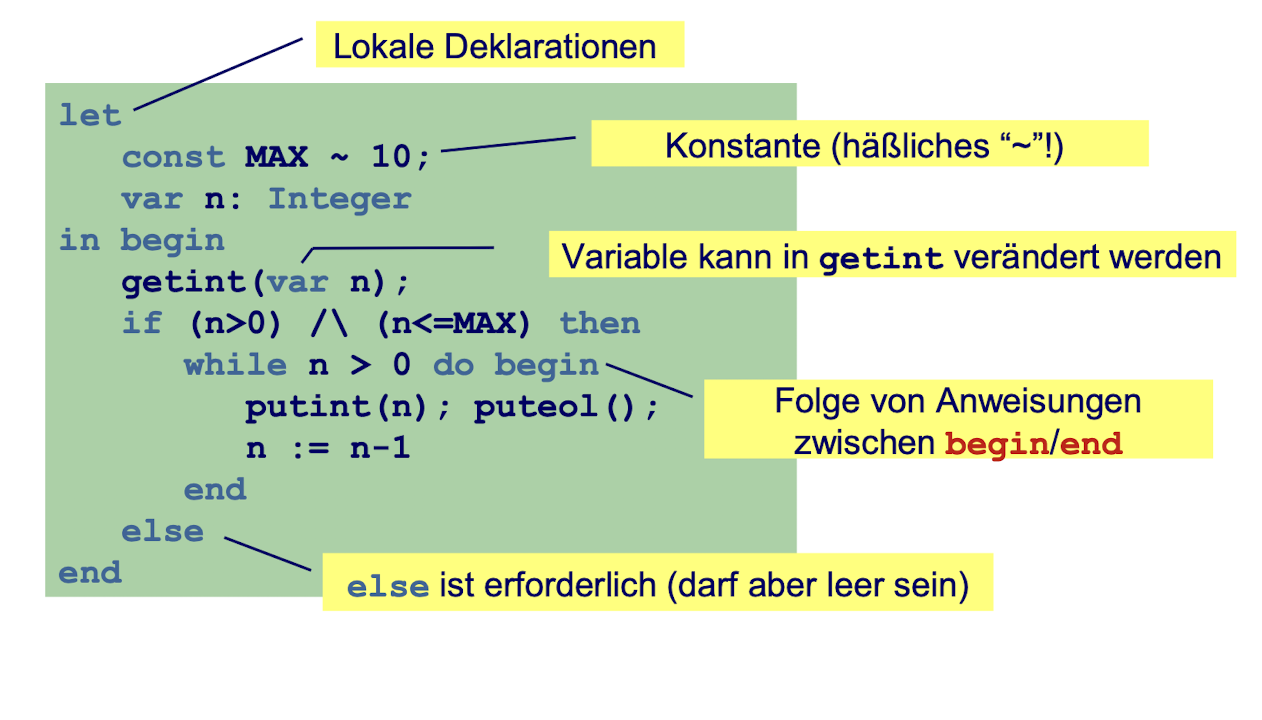
\includegraphics[width=0.5\linewidth]{/Users/lenavo/Desktop/3.Semester/Compilerbau/img/comp9.png}
    \caption{Mini-Triangle}
    \label{fig:enter-label}
\end{figure}
\subsection{Terminologie}
\textbf{\hl{Phrase:}} von einem gegebenen Nicht-Terminalsymbol herleitbare Kette von Terminalsymbolen\\[3mm]
\textbf{\hl{Satz:}} S-Phrase, wobei $S$ das Startsymbol der CFG ist
\begin{figure}[h]
    \centering
    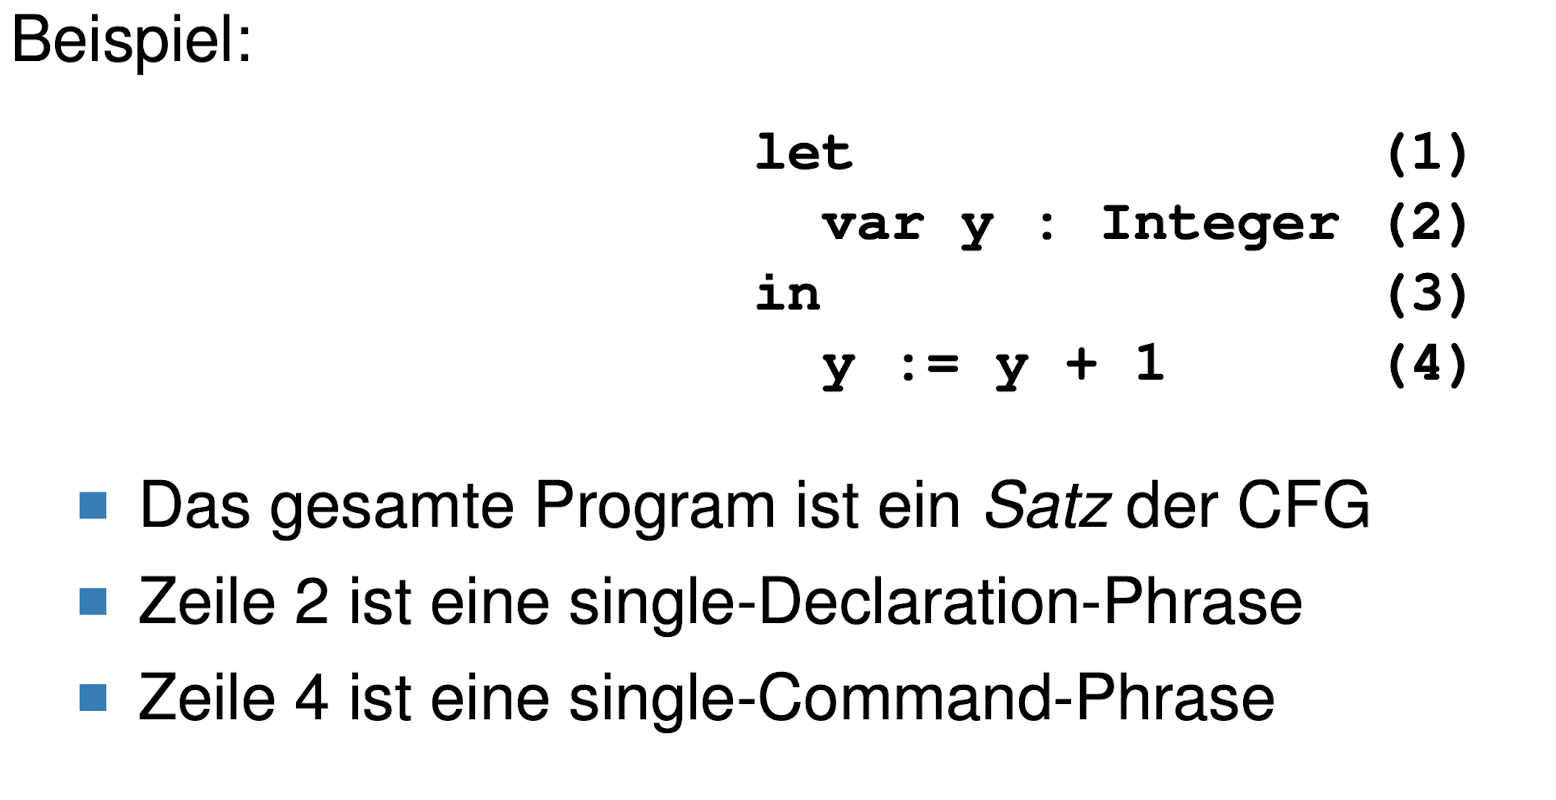
\includegraphics[width=0.5\linewidth]{/Users/lenavo/Desktop/3.Semester/Compilerbau/img/comp10.png}
    \caption{Beispiel}
    \label{fig:enter-label}
\end{figure}
\end{document}  
